\begin{solution}
\def\uhat{\widehat{u}}
\begin{enumerate}
\item {[4 points]} We can compute that, for $n=1,2,\ldots$,
\[
\psi_n'(x)=\sqrt{2} \left(n-{1\over 2}\right) \pi \cos\left(\left(n-{1\over 2}\right) \pi x\right)
\]
and
\[
\psi_n''(x)=-\sqrt{2} \left(n-{1\over 2}\right)^2 \pi^2 \sin\left(\left(n-{1\over 2}\right) \pi x\right)
\]
and so
\[
L\psi_n=-\psi_n''=\left(n-{1\over 2}\right)^2 \pi^2\psi_n.
\]
Hence,
\[
\lambda_n = \left(n-{1\over 2}\right)^2 \pi^2\mbox{ for } n = 1, 2, \ldots.
\]

\item {[8 points]} Let $f\in C[0,1]$ be defined by $f(x)=x+\sin(\pi x)$. Then $\tilde{u}$ is the solution to $L\tilde{u}=f$ and so the spectral method yields the series solution
\[
\tilde{u}(x)=\sum_{n=1}^\infty{\ip{f,\psi_n}\over\lambda_n}\psi_n(x).
\]
Now, for $k=1,2,\ldots$,
     \begin{eqnarray*} 
          \sqrt{2} \int_0^1 x \sin\left(\left(k-{1\over2}\right)\pi x\right) \, dx
                      &=& {\sqrt{2}\left(\left(k-{1\over2}\right)\pi\cos\left(\left(k-{1\over2}\right)\pi\right)+\sin\left(\left(k-{1\over2}\right)\pi\right)\right)
                               \over \left(k-{1\over2}\right)^2\pi^2}
\\
                      &=& {4\sqrt{2}\sin\left(\left(k-{1\over2}\right)\pi\right) \over \left(2k-1\right)^2\pi^2}
     \end{eqnarray*}
     and twice integrating by parts shows that
\begin{eqnarray*}
&&\sqrt{2} \int_0^1 \sin\left(\pi x\right) \sin\left(\left(k-{1\over2}\right)\pi x\right) \, dx 
\\
&=& {\sqrt{2}\left(\pi \cos\left(\pi\right)\sin\left(\left(k-{1\over2}\right)\pi\right) - \left(k-{1\over2}\right)\pi\sin\left(\pi\right)\cos\left(\left(k-{1\over2}\right)\pi\right)\right)
                    \over \left(k-{1\over2}\right)^2\pi^2-\pi^2}
\\
&=& -{\sqrt{2} \sin\left(\left(k-{1\over2}\right)\pi\right) \over \left(\left(k-{1\over2}\right)^2-1\right)\pi}.
\end{eqnarray*}
We put these pieces together to find that, for $k=1,2,\ldots$,
\begin{eqnarray*}
\ip{f, \psi_k} &=& {4\sqrt{2}\sin\left(\left(k-{1\over2}\right)\pi\right) \over \left(2k-1\right)^2\pi^2}-{\sqrt{2} \sin\left(\left(k-{1\over2}\right)\pi\right) \over \left(\left(k-{1\over2}\right)^2-1\right)\pi}
\\
&=& \sqrt{2}\sin\left(\left(k-{1\over2}\right)\pi\right)\left({4 \over \left(2k-1\right)^2\pi^2}-{1 \over \left(\left(k-{1\over2}\right)^2-1\right)\pi}\right)
\\
&=& \sqrt{2}\sin\left(\left(k-{1\over2}\right)\pi\right){4\left(\left(k-{1\over2}\right)^2-1\right)-\left(2k-1\right)^2\pi \over \left(2k-1\right)^2\left(\left(k-{1\over2}\right)^2-1\right)\pi^2}.
\end{eqnarray*}
The spectral method thus gives the formula
\[
     \tilde{u}(x) = \sum_{k=1}^\infty 2\sin\left(\left(k-{1\over2}\right)\pi\right){4\left(\left(k-{1\over2}\right)^2-1\right)-\left(2k-1\right)^2\pi \over \left(2k-1\right)^4\left(\left(k-{1\over2}\right)^2-1\right)\pi^4}\sin\left(\left(k-{1\over2}\right)\pi x\right).
\]
\item {[4 points]} Though not asked for in the question, the exact solution can be determined to be
\[ \tilde{u}(x) = {\sin(\pi x) \over \pi^2} -{x^3 \over 6} + {x\over 2} + {x\over \pi}.\]
The plots below compare the exact solution to the partial sums involving
1, 2, 3, and 20 terms.  The code that produced the plots follows.
\begin{center}
   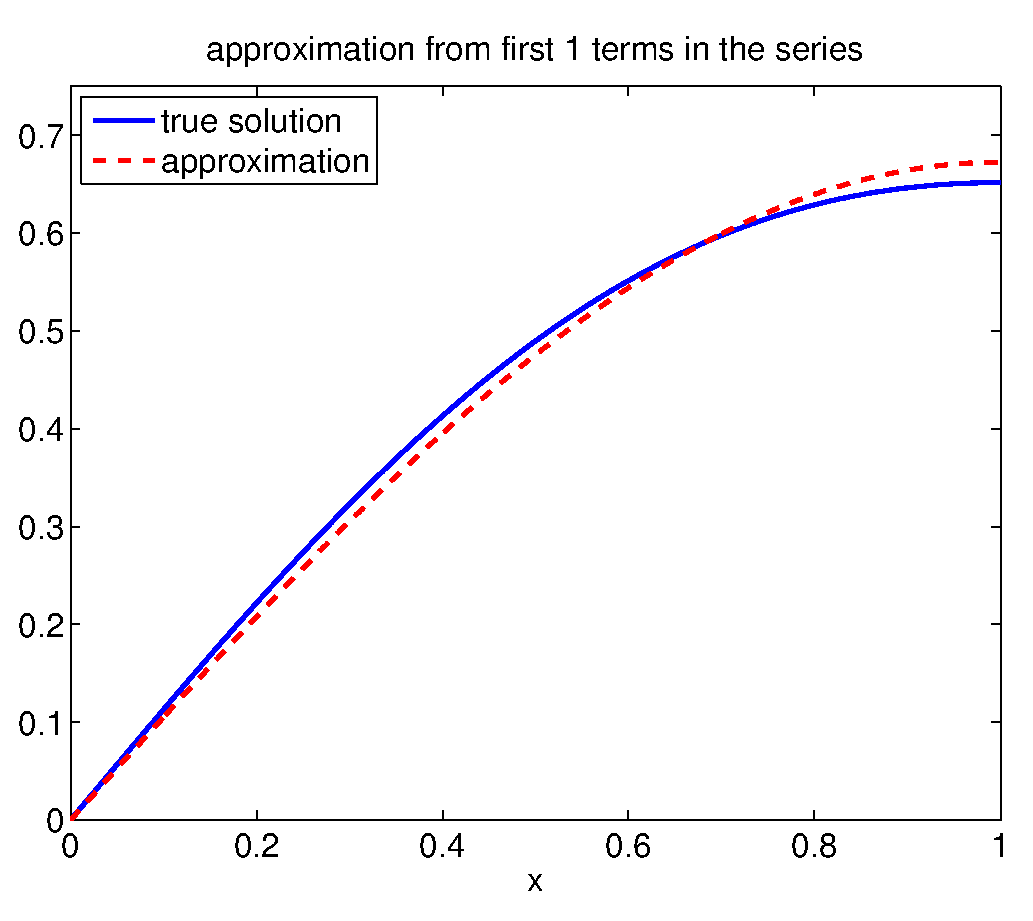
\includegraphics[scale=0.4]{bvps_1}\quad
   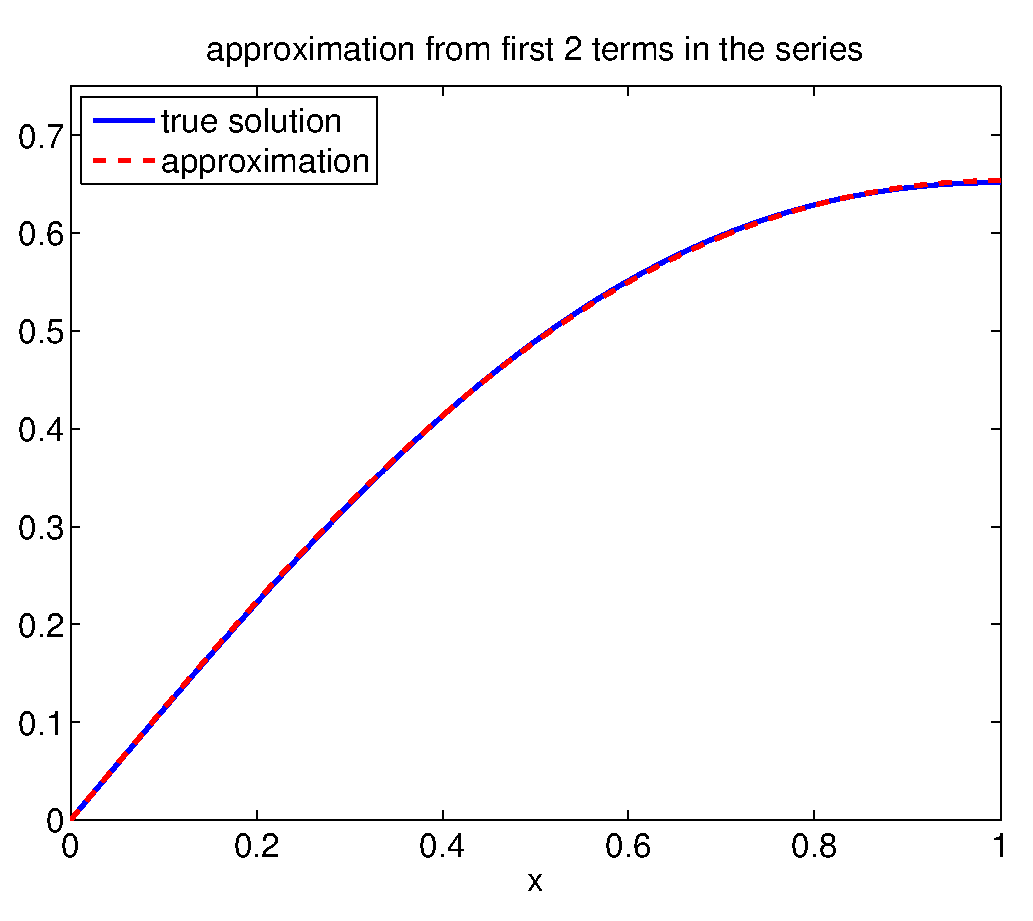
\includegraphics[scale=0.4]{bvps_2}

   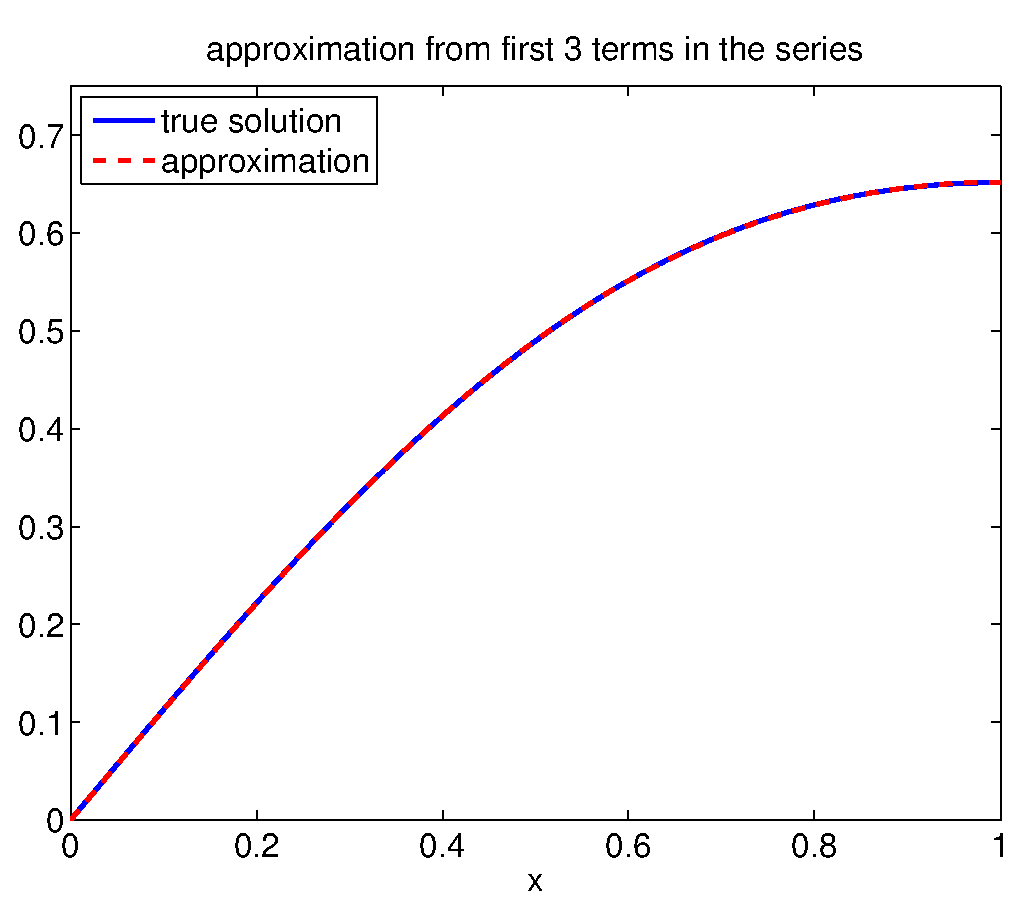
\includegraphics[scale=0.4]{bvps_3}\quad
   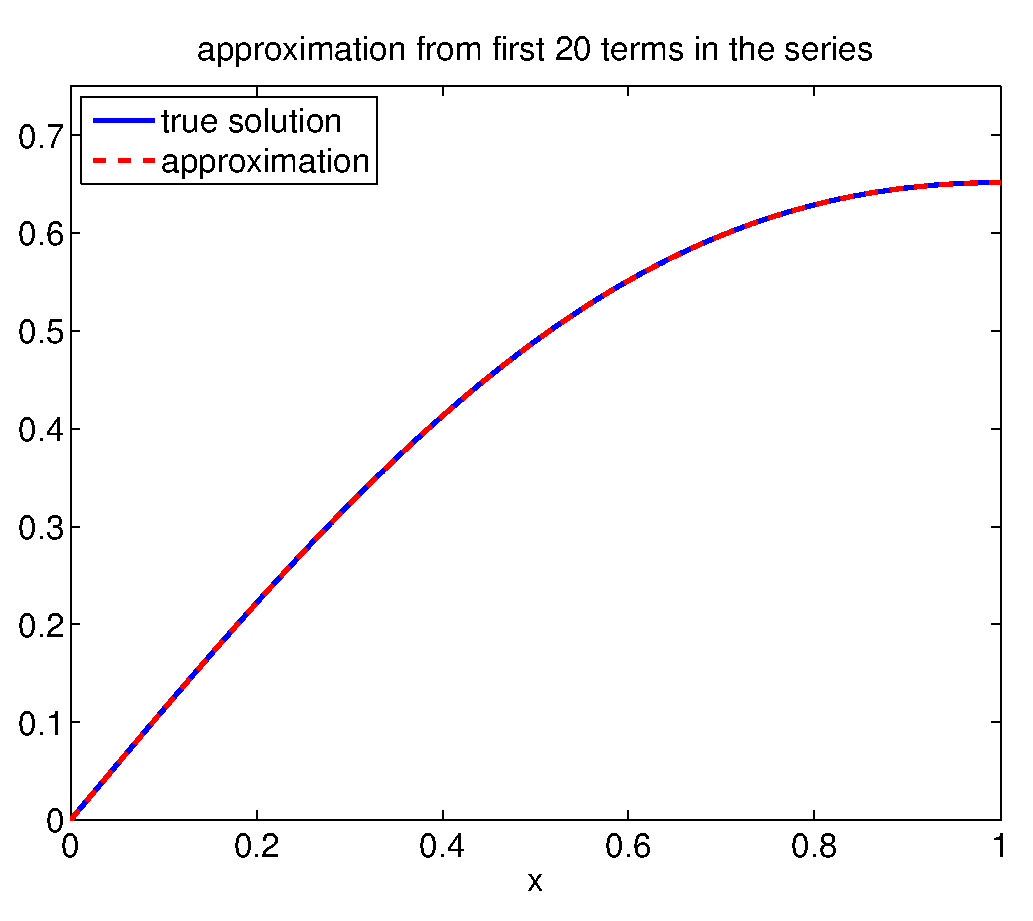
\includegraphics[scale=0.4]{bvps_20}
\end{center}

\lstinputlisting{HW28c.m}

\item {[5 points]} Let $\tilde{u}$ be the solution to $L\tilde{u}=f$ and let $w\in C^2[0,1]$ be such that
\[
-w''(x)=0,\quad0<x<1
\]
and
\[
w(0)=w'(1)=1.
\]
Then $u(x)=w(x)+\tilde{u}(x)$ will be such that
\[
-u''(x)=-w''(x)-\tilde{u}''(x)=0+f(x)=f(x);
\]
\[
u(0)=w(0)+\tilde{u}(0)=1+0=1;
\]
and
\[
u'(1)=w'(1)+\tilde{u}'(1)=1+0=1.
\]
Now, the general solution to
\[
-w''(x)=0
\]
is $w(x)=Ax+B$ where $A$ and $B$ are constants. Moreover, $w'(x)=A$ and so $w'(1)=1$ when $A=1$. Hence, $w(x)=x+B$ and so $w(0)=B$ and hence $w(0)=1$ when $B=1$. Consequently,
\[
w(x)=1+x
\]
and so
\[
u(x)=1+x+\tilde{u}(x).
\]
We can then use the series solution to $L\tilde{u}=f$ that we obtained in part (c) to obtain the series solution
\[
u(x)=1+x+\sum_{k=1}^\infty 2\sin\left(\left(k-{1\over2}\right)\pi\right){4\left(\left(k-{1\over2}\right)^2-1\right)-\left(2k-1\right)^2\pi \over \left(2k-1\right)^4\left(\left(k-{1\over2}\right)^2-1\right)\pi^4}\sin\left(\left(k-{1\over2}\right)\pi x\right)
\]
to the problem of finding $u\in C^2[0,1]$ such that
\[
-u''(x)=f(x),\quad0<x<1
\]
and
\[
u(0)=u'(1)=1.
\]

\item {[4 points]} Though not asked for in the question, the exact solution is
\[ u(x) = 1 + x + {\sin(\pi x) \over \pi^2} -{x^3 \over 6} + {x\over 2} + {x\over \pi}.\]
The plots below compare the exact solution to the partial sums involving
1, 2, 3, and 20 terms.  The code that produced the plots follows.
\begin{center}
   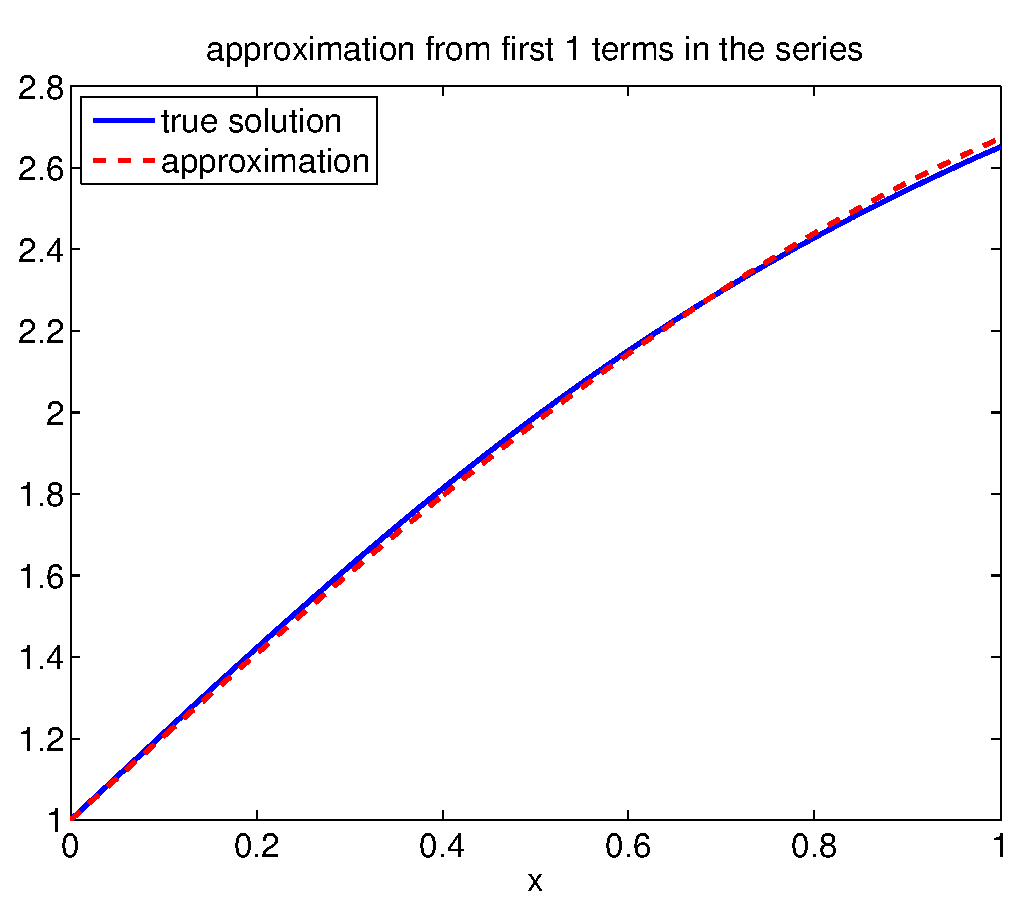
\includegraphics[scale=0.4]{bvpsin_1}\quad
   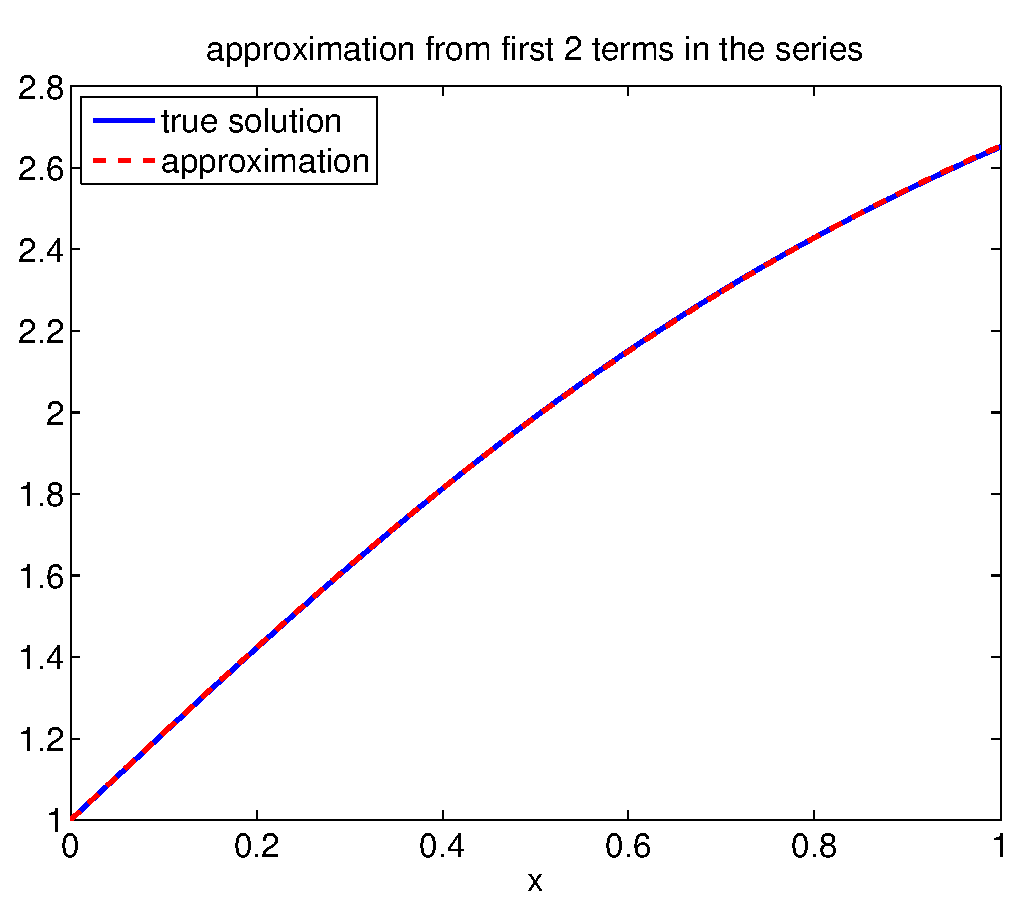
\includegraphics[scale=0.4]{bvpsin_2}

   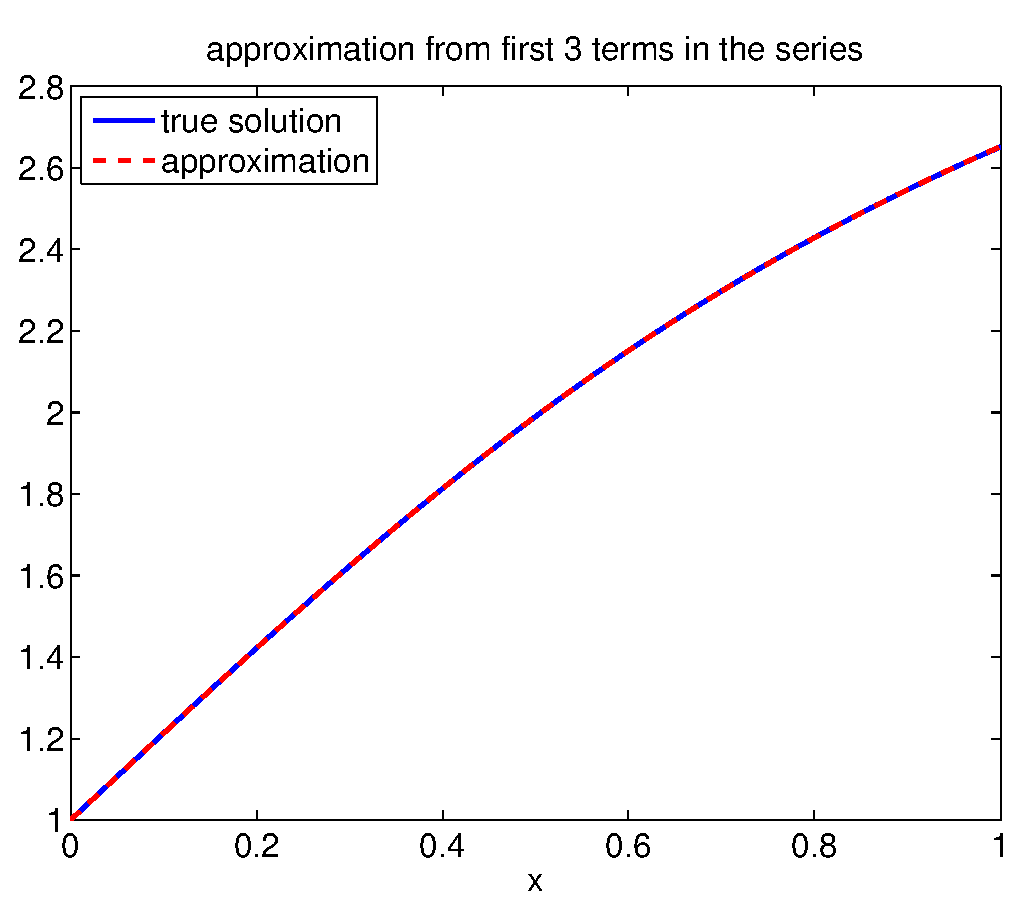
\includegraphics[scale=0.4]{bvpsin_3}\quad
   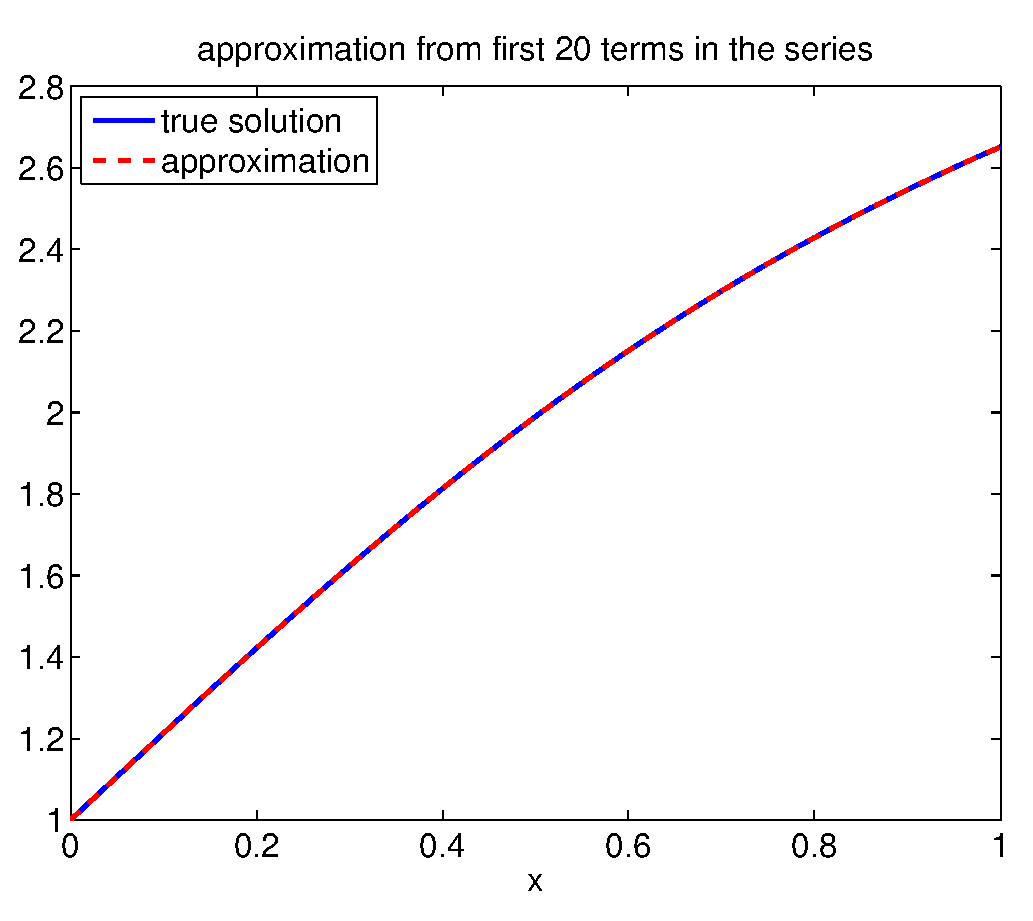
\includegraphics[scale=0.4]{bvpsin_20}
\end{center}

\lstinputlisting{HW28e.m}

\end{enumerate}
\end{solution}